\chapter{Accuracy Experiments}
\label{ch:results}

This chapter reproduces the two accuracy experiments the paper reports for
its offline protocol: the sensitivity of eALS to the missing-data weighting
parameters $c_0$ and $\alpha$ (the paper's Figure~1), and the convergence of
eALS against a uniform-weighting ablation (the paper's Figure~2, restricted
here to the two variants that isolate the effect this report cares about
most directly). All numbers below come from \texttt{results/weighting\_study.csv}
and \texttt{results/method\_comparison.csv}, produced by
\texttt{src/run\_experiments.py}, and are reported at $K=32$.

\section{Weighting the missing data}
\label{sec:weighting}

Section~\ref{sec:popweight} introduced two parameters governing how much
weight missing (unobserved) entries carry in the objective: $c_0$, the
overall strength of the penalty, and $\alpha$, which controls how much that
penalty is skewed towards popular items. Figure~\ref{fig:weighting_c0}
sweeps $c_0$ with $\alpha=0$ fixed (uniform weighting among missing
entries, only its overall magnitude varying).

\begin{figure}[H]
\centering
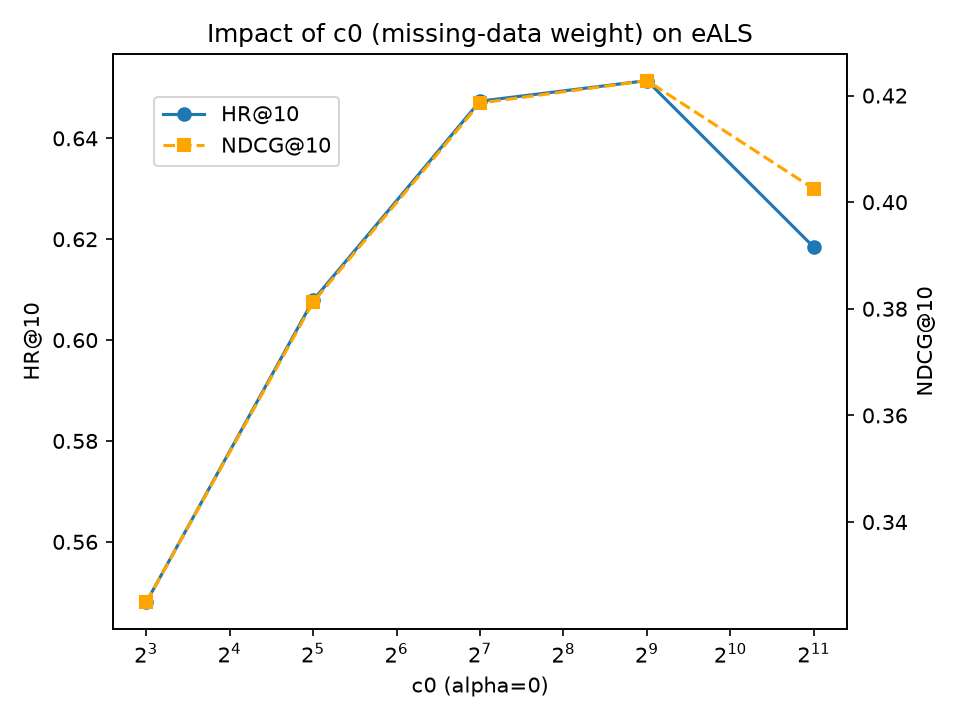
\includegraphics[width=0.65\textwidth]{figures/weighting_c0.png}
\caption{HR@10 and NDCG@10 as a function of $c_0$, with $\alpha=0$ (uniform
missing-data weighting). Peak performance at $c_0=512$.}
\label{fig:weighting_c0}
\end{figure}

The trend matches the paper closely: performance is poor when $c_0$ is
small (missing data contributes almost nothing to the loss, so the model
cannot distinguish ``never shown'' from ``actively disliked''), improves
sharply as $c_0$ grows, peaks, and then degrades again once the missing-data
term overwhelms the signal from the much smaller set of actually observed
interactions. On this dataset the peak sits at $c_0=512$ (HR@10 = 0.6514,
NDCG@10 = 0.4228), which happens to coincide exactly with the value the
paper itself reports as optimal for Amazon. That is a useful cross-check,
since $c_0$ is an absolute magnitude that in principle could have needed
rescaling for a differently-sized dataset.

\medskip
With $c_0$ fixed at 512, Figure~\ref{fig:weighting_alpha} sweeps $\alpha$,
which redistributes that fixed total weight towards more popular items as
$\alpha$ increases.

\begin{figure}[H]
\centering
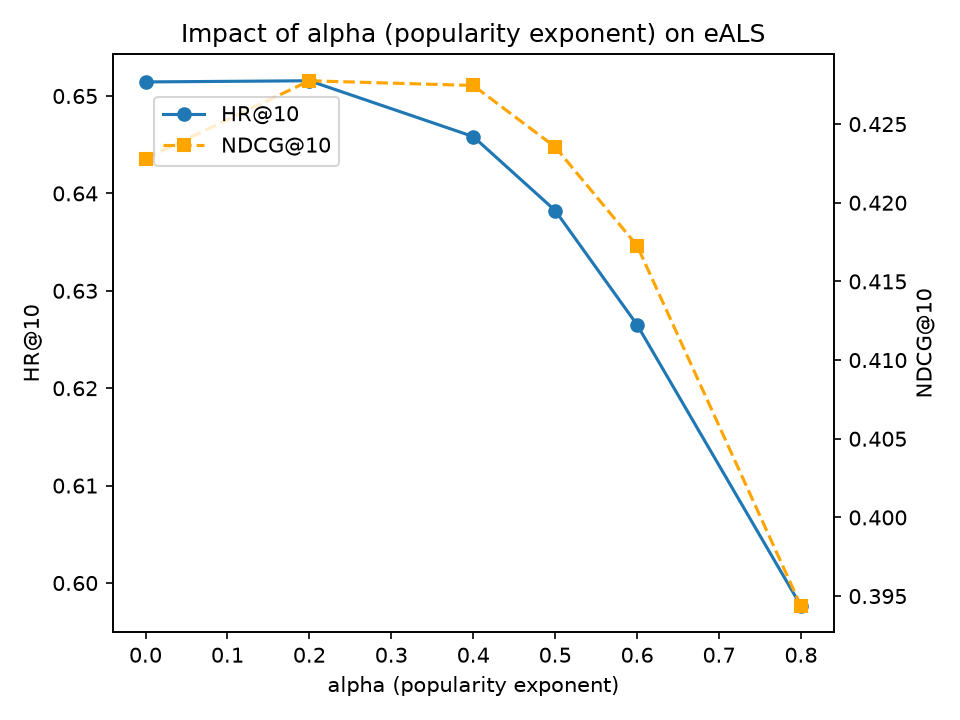
\includegraphics[width=0.65\textwidth]{figures/weighting_alpha.png}
\caption{HR@10 and NDCG@10 as a function of $\alpha$, with $c_0=512$. Best
NDCG@10 at $\alpha=0.2$.}
\label{fig:weighting_alpha}
\end{figure}

Here the result is close to, but not identical to, the paper's finding.
\citet{he2016eals} report a clear optimum around $\alpha=0.4$ for Amazon,
with a statistically significant improvement over $\alpha=0$ (uniform
weighting). On this dataset, NDCG@10 peaks at $\alpha=0.2$
(NDCG@10 = 0.4278, HR@10 = 0.6516), and $\alpha=0$ (NDCG@10 = 0.4228) is
already close to that peak and slightly ahead of $\alpha=0.4$
(NDCG@10 = 0.4275, effectively tied with $\alpha=0.2$ within the noise one
would expect from a single training run) and clearly ahead of $\alpha=0.6$
and $\alpha=0.8$, which both degrade markedly. The qualitative shape of the
curve is preserved, a mild optimum somewhere in $(0, 0.5)$ followed by a
drop-off for large $\alpha$, but the exact location of the optimum is not,
and popularity weighting's advantage over plain uniform
weighting is much smaller here than the paper reports. Section~\ref{sec:weaknesses}
discusses the most likely reasons for this, chief among them the
roughly $5\times$ smaller and differently-curated dataset used here
compared to the paper's.

\section{Convergence}
\label{sec:convergence}

Figure~\ref{fig:convergence} tracks HR@10 and NDCG@10 across 15 training
iterations for two configurations that isolate the effect of popularity
weighting while holding the solver fixed: eALS with $\alpha=0.4$ (the
paper's recommended popularity-aware weighting) against eALS with
$\alpha=0$ (Hu et al.'s uniform-weighting objective, solved with the same
element-wise solver, which makes this an ablation of the weighting scheme
alone rather than a comparison between two different algorithms).

\begin{figure}[H]
\centering
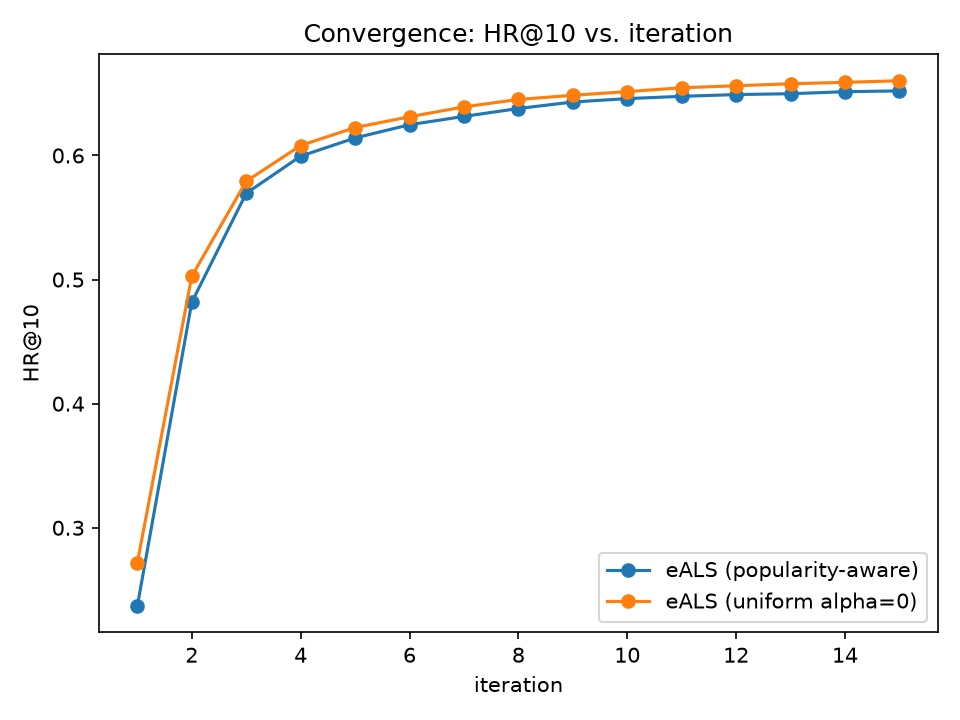
\includegraphics[width=0.65\textwidth]{figures/convergence_HR_at_10.png}
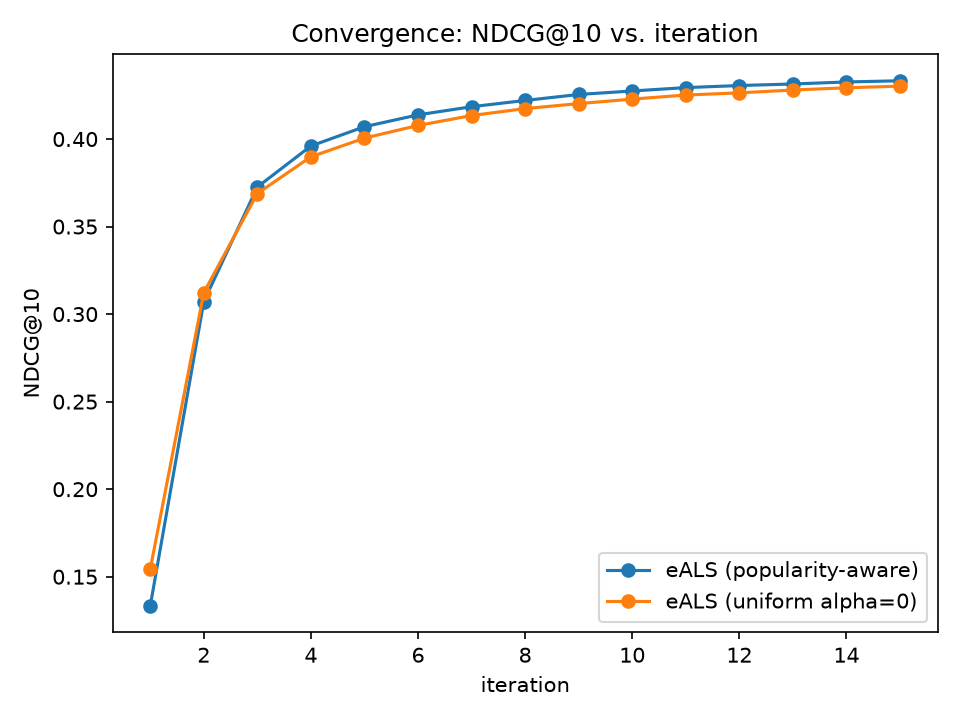
\includegraphics[width=0.65\textwidth]{figures/convergence_NDCG_at_10.png}
\caption{HR@10 (top) and NDCG@10 (bottom) versus training iteration, for
popularity-aware ($\alpha=0.4$) and uniform ($\alpha=0$) weighting.}
\label{fig:convergence}
\end{figure}

Both variants converge fast and to essentially the same place: HR@10 jumps
from roughly 0.24-0.27 after a single iteration to above 0.60 within five
iterations, and both curves flatten out by iteration 10-12, ending at
HR@10 = 0.652 / NDCG@10 = 0.433 for the popularity-aware variant and
HR@10 = 0.660 / NDCG@10 = 0.430 for the uniform variant. The difference is
small enough that it should not be read as one variant being reliably
better than the other on this dataset, consistent with the narrow gap
already seen in Figure~\ref{fig:weighting_alpha}. What the paper reports
qualitatively also holds here: eALS reaches a good solution quickly because
each coordinate update is an exact minimizer of the objective given the
current state of every other coordinate, rather than a step in the
direction of steepest descent. There is no learning rate to tune and no
risk of overshooting, which is precisely the property the paper credits
for eALS's fast, learning-rate-free convergence compared to gradient-based
alternatives such as RCD \citep{devooght2015dynamic} or BPR
\citep{rendle2009bpr}.

\medskip
The logged wall-clock time for the full 15-iteration run happened to differ
between the two configurations (400\,s for $\alpha=0.4$ versus 297\,s for
$\alpha=0$), even though the two runs perform the exact same sequence of
arithmetic operations: $\alpha$ only changes the numeric values fed into
identical update formulas, not the amount of work done. This gap is most
plausibly measurement noise from running two multi-minute jobs sequentially
on a shared machine (JIT warm-up, OS-level caching, background load) rather
than a real algorithmic effect, and it should not be over-interpreted. Note
also that these per-iteration times are not comparable to the pure
training-only timings in Chapter~\ref{ch:scalability}: computing
HR@10/NDCG@10 after every single iteration, to plot Figure~\ref{fig:convergence},
adds a full evaluation pass over all 33{,}326 test users on top of the
training step itself, which is why this experiment averages roughly 27\,s
per iteration at $K=32$ while Section~\ref{sec:scale_k} reports 11.5\,s for
training alone at the same $K$. Chapter~\ref{ch:scalability}'s figures,
which measure training time only and average over repeated short runs
specifically designed to control for scheduling variance, are the more
reliable source for anything to do with training cost in isolation.
